\documentclass{article}

\usepackage{../packages}

\graphicspath{{./figures}}


\begin{document}
\begin{titlepage}
\begin{center}
	
\includegraphics[scale=0.7]{logo.png}

	\vspace*{4cm}
	\textbf{Bazy danych\\ Laboratorium}

	\vspace{1.5cm}
	\textit{Zapytania DDL SQL Oracle 2}

	\vspace{1.5cm}
	\textbf{Stanislau Antanovich}\\
	nr. indeksu: 173590\\
	gr. lab: L04

	\vspace{4.5cm}
\end{center}
\end{titlepage}

\tableofcontents
\listoffigures
\lstlistoflistings

\newpage
 
\section{Wprowadzenie}

\subsection{Cel ćwiczenia}

\subsection{Przygotowanie}

\section{Realizacja}

\begin{enumerate}
\item Tworzenie i wywołanie procedury \textbf{dodaj\_etat} pozwalającej na dodanie nowego etatu

\begin{lstlisting}[style=SQL, caption=\textit{Tworzenie i wywołanie procedury \textbf{dodaj\_etat}}]
CREATE PROCEDURE dodaj_etat(
	p_id IN NUMBER,
	p_etat IN VARCHAR
) AS
BEGIN
	INSERT INTO ETATY (ID_ETATU, ETAT) VALUES (p_id, p_etat);
	COMMIT;
END dodaj_etat;

EXEC dodaj_etat(673, 'EMPLOYEE')
\end{lstlisting}

		\begin{figure}[H]
			\centering
			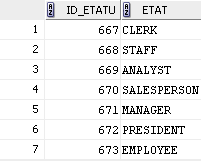
\includegraphics[scale=1.2]{zadanie1.png}
			\caption{\textit{Tworzenie i wywołanie procedury \textbf{dodaj\_etat}}}
		\end{figure}

\item Tworzenie i wywołanie procedury \textbf{usun\_pracownika} pozwalającej na usunięcie pracownika na podstawie podanego id(parametr wejściowy)

	\begin{lstlisting}[style=SQL, caption=\textit{Tworzenie i wywołanie procedury \textbf{usun\_pracownika}}]
	\end{lstlisting}

		\begin{figure}[H]
			\centering
			\caption{\textit{Tworzenie i wywołanie procedury \textbf{usun\_pracownika}}}
		\end{figure}

\item Tworzenie i wywołanie proceduty \textbf{edytuj\_pracownika} pozwalającej na edytowanie kolumn pracownika na podstawie podanych parametrów

	\begin{lstlisting}[style=SQL, caption=\textit{Tworzenie i wywołanie procedury \textbf{edytuj\_pracownika}}]
	\end{lstlisting}

		\begin{figure}[H]
			\centering
			\caption{\textit{Tworzenie i wywołanie procedury \textbf{edytuj\_pracownika}}}
		\end{figure}

\item Modyfikacja procedury \textbf{dodaj\_etat} w taki sposób, aby uniknąć wystąpienia duplikującego się rekordu.

	\begin{lstlisting}[style=SQL, caption=\textit{Modyfikacja procedury \textbf{dodaj\_etat}}]
	\end{lstlisting}

		\begin{figure}[H]
			\centering
			\caption{\textit{Modyfikacja procedury \textbf{dodaj\_etat}}}
		\end{figure}

\item Zaproponowana funkcja \textbf{srednia\_pensja}, która zwraca średnią pensję wszystkich pracowników
	
	\begin{lstlisting}[style=SQL, caption=\textit{Zaproponowana funckja \textbf{srednia\_pensja}}]
	\end{lstlisting}

		\begin{figure}[H]
			\centering
			\caption{\textit{Zaproponowana funkcja \textbf{srednia\_pensja}}}
		\end{figure}

\item Zaproponowana funkcja \textbf{zmien\_prowizje}, która umożliwi na podstawie id pracownika zmienić jego prowizję. W przypadku wprowadzonej wartości poniżej zera funkcja ma zgłosić odpowiedni wyjątek

	\begin{lstlisting}[style=SQL, caption=\textit{Zaproponowana funkcja \textbf{zmien\_prowizje}}]
	\end{lstlisting}

	\begin{figure}[H]
		\centering
		\caption{\textit{Zaproponowana funkcja \textbf{zmien\_prowizje}}}
	\end{figure}

\item Zaproponowana funkcja \textbf{ilosc\_pracownicy\_z\_pensja} umożliwiająca zwrócenie ilości pracowników, których pensja mieści się w podanym przedziale <min;max>

	\begin{lstlisting}[style=SQL, caption=\textit{Zaproponowana funkcja \textbf{ilosc\_pracownicy\_z\_pensja}}]
	\end{lstlisting}

	\begin{figure}[H]
		\centering
		\caption{\textit{Zaproponowana funkcja \textbf{ilosc\_pracownicy\_z\_pensja}}}
	\end{figure}

\item Zaproponowana funkcja \textbf{zwieksz\_pensje}, która na podstawie id pracownika zmienia wartość kolumny pensja zgodnie z zasadami:
\begin{itemize}
\item jeżeli pracownik nie ma zwierzchnika jego pensja nie ulega zmianie
\item jeżeli pracownik ma zwierzchnika, ale ma prowizje, pensja zwiększa się o wartość 100
\item jeżeli pracownik ma zwierzchnika, ale nie ma prowizji, pensja zwiększa się o 10\%
\item funkcja zwraca nową pensję jako wartość
\end{itemize}

\begin{lstlisting}[style=SQL, caption=\textit{Zaproponowana funkcja \textbf{zwieksz\_pensje}}]
\end{lstlisting}

\begin{figure}[H]
	\centering
	\caption{\textit{Zaproponowana funkcja \textbf{zwieksz\_pensje}}}
\end{figure}

\item Wywołanie komendy usunięcia dowolnej procedury i funkcji
	
	\begin{lstlisting}[style=SQL, caption=\textit{Wywołanie komendy usunięcia dowolnej procedury i funkcji}]
	\end{lstlisting}

	\begin{figure}[H]
		\centering
		\caption{\textit{Wywołanie komendy usunięcia dowolnej procedury i funkcji}}
	\end{figure}

\item Zaproponowany typ pozwalający przechowywać dane obiektu \textbf{ETAT} oraz tabelę etatów

	\begin{lstlisting}[style=SQL, caption=\textit{Zaproponowany typ pozwalający przechowywać dane obiektu \textbf{ETAT} oraz tabelę etatów}]
	\end{lstlisting}
	
	\begin{figure}[H]
		\centering
		\caption{\textit{Zaproponowany typ pozwalający przechowywać dane obiektu \textbf{ETAT} oraz tabelę etatów}}
	\end{figure}

\item Zaproponowana funkcja zwracająca tabelę z danymi obiektów \textbf{ETAT} zaproponowanymi w poprzedznim zadaniu. Dane(id, etat):(`100',`stażysta'),(`101',`junior'),(`102',`medium'),(`103',`master')

	\begin{lstlisting}[style=SQL, caption=\textit{Zaproponowana funkcja zwracająca tabelę z danymi obiektów \textbf{ETAT}}]
	\end{lstlisting}

	\begin{figure}[H]
		\centering
		\caption{\textit{Zaproponowana funkcja zwracająca tabelę z danymi obiektów \textbf{ETAT}}}
	\end{figure}
\item Zaproponowana funkcja \textbf{zwroc\_etaty}, która zwraca wszystkie etaty w formie tabeli

	\begin{lstlisting}[style=SQL, caption=\textit{Zaproponowana funkcja \textbf{zwroc\_etaty}}]
	\end{lstlisting}

	\begin{figure}[H]
		\centering
		\caption{\textit{Zaproponowana funkcja \textbf{zwroc\_etaty}}}
	\end{figure}
\end{enumerate}

\section{Wnioski}


\end{document}
